In this section I will first define and discuss the state of reproducibility in science across a range of domains, and
explore several specific examples. Next, I will discuss the role that software reusability and numerical stability
play in these problems, and advances which have been made in each of these fields. I will then approach neuroimaging,
with a brief overview of the field and commonly used methods that are of relevance, finally presenting several case
studies in neuroimaging to demonstrate the necessity of exploring numerical stability in this space.

\subsection{Scientific Reproducibility}
At the heart of science is the ability for researchers to build upon previous work, incrementally advancing a given
field of research~\cite{salmon1999introduction,platt1964strong}. Despite being accepted as a cornerstone for progress,
there is not a fully unified vocabulary around this
practice~\cite{plesser2018reproducibility,patil2019visual,goodman2016does}. Definitions have emerged to serve specific
communities tackling issues of reproducibility, such as The Association for Computing Machinery which defines
reproducibility as the ability to re-obtain a measure with stated quality and precision using an identical experimental
setup when carried out by a different team in a different location~\cite{acm_2020}. In the case of life sciences, this
definition has limited use since the samples being measured (e.g. human participants) or equipment used (e.g. exact
imaging apparatus from the same manufacturer) is difficult or impossible to replicate. In these cases, a distinction in
the level of reproducibility is often drawn with milestones corresponding to the ability to reproduce the methods used,
the ability to obtain the same or equivalent results, and the ability to draw equivalent inferences from the results
obtained~\cite{plesser2018reproducibility}.

In an effort to increase clarity around this topic and handfuls of overlapping definitions, there have been recent
efforts to visualize the intentions and slight conceptual differences across each~\cite{patil2019visual}. Here, a
distinction is made from reproducibility and replicability. Reproducibility in this case is defined as the ability to
exactly re-run the analysis using the existing data and tools, but is performed by a unique analyst. Replicability then
describes the ability to successfully re-do the experiment, including new data collection, experimenters, and software,
but ultimately arriving at the same claim. These definitions have practical value in the life sciences as they allow for
the differentiation between a claim remaining unchanged in either the same or differing experimental configurations and
equipment. The definitions presented here, often referred to colloquially as ``Peng's Reproducibility'', will be those
referred to throughout this thesis.

In addition to the definitions of reproducibility and replicability accepted above, I will refer to an additional term
in this space: reusability, which simply refers to the ability of being able to ``hit go'' on the analysis
subsequent to its original execution. This definition closely matches a definition of reproducibility mentioned above,
but no analog exists within the Peng framework, so it is added here for clarity.

With a rich and growing space of conceptual frameworks through which reusability, reproducibility, and
replicability can be evaluated, it is perhaps self-evident that the level of trustworthiness across many disciplines
has recently become a topic of interest. I will now introduce the so-called ``Reproducibility Crisis'', an umbrella
phrase which captures this movement, and highlight its relevance in both psychological and neurological sciences,
serving as motivation for the work carried out in this thesis.

\subsection{The Reproducibility Crisis}

The reproducibility of findings has long been a topic of concern to researchers in the life
sciences~\cite{ioannidis2005most,begley2012raise,prinz2011believe,mcnutt2014reproducibility}. However, several recent
initiatives have brought this somewhat fringe topic into an area of broad concern. In 2015, the Open Science
Collaboration~\cite{open2015estimating} organized an attempted replication of $100$ recent research papers in
psychology. Their result, showing that approximately two-thirds of the studies failed to replicate, was swept up by
mainstream media and proclaimed a crisis.

In an effort to characterize the so-called crisis, Nature conducted a survey of $1,500$ scientists across a wide
range of disciplines, probing their beliefs about the reproducibility of science in their field. This study found that
$90\%$ of respondents felt that their field was in some level of crisis~\cite{baker20161}, and studies exploring
possible causes or proposing solutions to the so-called crisis have continued to trend in the years since.
Unsurprisingly, this phenomenon has been characterized from a number of different directions, even within a given
discipline. In neuroscience, for example, statistical power has long been believed to be a key culprit for
irreproducibility~\cite{button2013power}; a meta-analytic study of findings in literature estimated a median power of
$21\%$. This work, however, assumed the robustness of data and methods used throughout the studies, and performed a
purely statistical evaluation, so any inconsistencies in the analytical methods used may in reality lead to an even
lower statistical power across published results.

In neuroimaging, studies began to dive deeper into the intermediate processing methods and explored their compounded
effect on null hypothesis significance testing. A study evaluating the accuracy of significance testing frameworks within
commonly used libraries for the analysis of functional MRI (fMRI) data found that under certain conditions false-positive
rates were as high as $70\%$~\cite{eklund2016cluster}. While the presentation of this result may misleadingly construe an
inflated significance of these errors (see associated
letters\footnote{\url{https://www.pnas.org/content/114/17/E3368}}\footnote{\url{https://www.pnas.org/content/114/17/E3370}}
and correction\footnote{\url{https://www.pnas.org/content/113/33/E4929}}), undeniable attributes of these findings are
both that a) there is considerable variability in the quality of tools under certain conditions and b) there are
often-dramatic differences between supposedly-equivalent software libraries. The impact that cross-library differences have
on analytical workflows was well summarized in an attempted replication of experiments on real fMRI
datasets~\cite{bowring2019exploring}, which showed that not only do the tools produce qualitatively different results,
but could sometimes lead to diverging conclusions.

In all cases of limited reproducibility presented above, analyses were chosen to be evaluated explicitly because they
could be re-executed across slightly different conditions. While all published methods, such as software written to
produce the result associated with a given paper, would continue to function in an ideal world, in practice this is not
the case. A study exploring published papers in computer science found that of $600$ papers which were analyzed,
approximately only $200$ were able to weakly replicate~\cite{collberg2016repeatability}. In many cases, this was due to
inadequate description of the specific implementations, environments, or how tools were applied, while in others, it was
likely due to the commonly accepted phenomenon of ``Software Aging''~\cite{parnas1994software}. Regardless of the specific
causes, this inability to re-execute workflows makes claims derived from these workflows irreproducible at the most
fundamental level. Prior to exploring possible numerical underpinnings behind reproducibility, it is essential to ensure
the reusability of analyses. The following section will discuss advances made prior to this thesis which facilitate
the construction and distribution of re-executable scientific workflows.

\subsection{Software Reusability}
There are a number of factors which limit the re-executability or reuse of scientific workflows, including incomplete specification
of processing detail or lack of data and tool availability~\cite{ioannidis2009repeatability}. While the public sharing
and dissemination of data may not always be possible in the life sciences due to concerns around ethics or the informed
consent of participants~\cite{ross2018ethical,duke2013ethics}, there exist practical guides which can help researchers
overcome this hurdle in certain cases (e.g. for neuroimaging~\cite{brakewood2013ethics} and
psychology~\cite{meyer2018practical}). Given that ethical barriers should not exist limiting the reusability of
software, this section will focus on tangible efforts which have been made to increase the re-executability of
scientific pipelines.

\subsubsection{Virtual Environments}
The configuration of tools and software environments is a necessary step prior to the execution of computational
workflows. While authors set up their computational environments prior to carrying out experiments, these
configurations are often left undocumented in published manuscripts, leaving readers with the daunting task of
determining what versions of libraries were used and their dependencies~\cite{robles2010replicating}. However, this is
not only an inconvenience but becomes scientifically troublesome when considering the reality that distinct software
versions by design lead to incrementally different interfaces and results~\cite{raymond1997cathedral}. In programming
languages such as Python~\cite{oliphant2007python}, packages may contain information strictly defining their
requirements. However, these definitions are limited to capturing the dependencies written within the same language,
and are often written with version ``bounds'' (i.e. requires package X with version $\geq 1.0$), to simplify the
interoperability between libraries.

Traditionally, the issue of environment configuration has been solved through the use of Virtual Machines
(VMs)~\cite{smith2005virtual}. VMs are a method for packaging and sharing tools that are pre-installed in an executable
environment which can be run across computers. A drawback of these machines is that they are often require considerable
storage and computational overhead, as they contain complete operating systems which must be launched in virtualized
hardware, limiting their portability. Over the last few years, techniques for the virtual encapsulation of tools have
shifted towards a ``container'' approach, which does not suffer from similar overheads. Container environments,
made accessible primarily through Docker~\cite{merkel2014docker} and Singularity~\cite{kurtzer2017singularity}, rely on
the Linux kernel and other libraries of the host operating system, leading to smaller bundles that are less computationally
expensive to run. While containers are not a perfect solution that guarantee reusability\footnote{Due to problems which
may arise by violating some of the best-practices described here:
\url{https://developers.redhat.com/blog/2016/02/24/10-things-to-avoid-in-docker-containers/}}, they are an important
advancement which greatly increases the ability to distribute and consume scientific software, and provide a salve
against the problem of software aging.

\subsubsection{Tool \& Analysis Descriptions Standards}
Beyond tool configuration, the most fundamental components of re-executability are a clear characterization of the
tool(s) being run and the arguments or inputs provided to them. Despite this, there is no universally accepted
description standard for software. In practice, grassroots standards often emerge by necessity in a given domain, and
gain local adoption. In the case of neuroimaging, such standards include Brain Imaging Data Structure applications
(BIDS apps)~\cite{gorgolewski2017bids} and Boutiques~\cite{Glatard2018-tu}, each of which takes a distinct approach to
this problem.

The Brain Imaging Data Structure defines an organization standard for neuroimaging datasets, with the goal of lowering
the barrier to their sharing, interpretation, and inter-operation~\cite{gorgolewski2016brain}. Accordingly, the BIDS
app standard emerged as a \textit{prescriptive} standard that dictates how tools should interact with these
datasets~\cite{gorgolewski2017bids}. This standard requires that a set of base arguments must be supported and accepted
by tools: the location of the dataset, the location at which outputs should be placed, and the analysis level (e.g.
for the analysis of an individual versus the analysis of a group). This standard also prescribes several optional
arguments, such as allowing for the indication of a subset of subjects selected for analysis. However, a key limitation
of this standard is that beyond the initial prescription of arguments there is no definition or description of how
subsequent arguments that may be relevant for a given tool should be defined or documented. The BIDS app standard
dramatically simplifies performing an analysis pipeline with default behaviour, but this lack of additional description
and no provenance definition to keep analysis records makes it an incomplete solution for software re-use when
implemented at the barest level.

Boutiques facilitates re-executability through a \textit{descriptive} standard which requires software developers to
create a rich metadata record summarizing the arguments and function of their tools~\cite{Glatard2018-tu}. This standard
supports a wide range of command-line tools, and is supported by a library which directly manages the execution of
described tools alongside validation of inputs (e.g. ensuring two mutually-exclusive options are not provided) and
provenance capture. However, while the added complexity of Boutiques leads to more rich descriptions and facilitates
more complete tool re-use, this complexity also makes the standard considerably less accessible.

Other standards have been developed around neuroimaging which promote the capture of rich execution records, such as
the NeuroImaging Data Model~\cite{maumet2016sharing}, or foster the construction of workflows and the distributed
execution of tools, such as CBRAIN~\cite{maumet2016sharing}, LONI Pipeline~\cite{rex2003loni}, and
Nipype~\cite{gorgolewski2011nipype}. While these tools provide a rich set of features and techniques to improve the
re-executability of software, prior to this thesis there was no single tool in the neuroimaging space which harmonized
software virtualization, command-line tool descriptions, and provenance capture that supported the iterative
development and deployment of analysis pipelines across high performance computing systems.

\subsection{Numerical Stability}
\label{sec:bg_stab}
In cases where the re-execution of software can be attempted and reproduction of claims can be tested, there are myriad
possible sources of observed variability between results. While some of these may be avoided when following best
practices~\cite{prlic2012ten}, such as the dependence of an analysis on a pseudo-random number, there are algorithmic
properties which may persistently affect outcomes and would benefit from characterization. One such property is the
numerical stability of an algorithm or tool~\cite{higham2002accuracy}. While there are various theoretical and empirical
techniques used for evaluating stability, each conceptually refers to stability as measure of sensitivity to small
perturbations. Issues in stability emerge for one of two reasons: the evaluation of poorly conditioned functions (i.e.
those containing or nearby singularities), or the accumulation and propagation of numerical error~\cite{higham2002accuracy}.

In the case of poorly conditioned functions, instability may often be detected both theoretically and empirically. One
such measure for evaluating this is the ``condition number'' of a matrix or function~\cite{belsley2005regression}. While
the mathematical form can be simplified for different contexts (i.e. matrices or linear functions), its general
definition ultimately describes the worst-case error in the output for a relative change in input, as that change to input
asymptotically approaches $0$~\cite{belsley2005regression}. This allows functions to be evaluated with respect to
their sensitivity to minor perturbations of their inputs, where a smaller condition number refers to smaller effect of
perturbations.

While the condition number of a function can in some cases refer to its practical robustness to perturbations, it ultimately
does not consider implementation so more accurately refers to how ``easy'' a function is to evaluate. In doing so, the
condition number relates two distinct components of the stability of a problem: the forward error and backward error. The
forward error is defined as the deviation of an output from the true result, while the backward error is defined as the
smallest change to an input such that the theoretical result matches the empirical result~\cite{higham2002accuracy}. The
condition number is bounded by a relationship of these values, such that it will always be greater than or equal to the
ratio of the forward error to the backward error~\cite{belsley2005regression}. In practice, forward and backward error are
often combined into a measure of mixed stability which evaluates how closely a solution matches another when the input is
perturbed slightly. In the case of problems where there is no ground-truth solution (e.g. alignment of an image to a
template) it is impossible to explore the forward error independently, while the backward error may be evaluated in certain
cases (e.g. if the approximation of a ground-truth alignment exists). Given that there is no guarantee that the backward
error is measurable for an arbitrary problem, the mixed stability is commonly evaluated (Figure~\ref{fig:stability}).

\begin{figure}[b!]
\centering
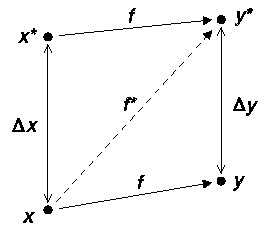
\includegraphics[width=0.4\textwidth]{./figs/forward_stab.pdf}
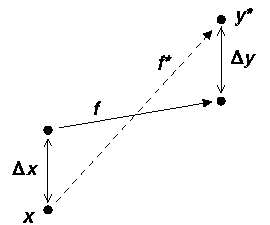
\includegraphics[width=0.4\textwidth]{./figs/mixed_stab.pdf}
\caption[Illustration of forward, backward, and mixed stability]{Illustration of forward and backward (left) or mixed
stability (right) definitions. Originally published in the public domain with the following captions. Left: Diagram showing
the forward error $\Delta y$ and the backward error $\Delta x$, and their relation to the exact solution map $f$ and the
numerical solution $f*$. Right: Mixed stability combines the concepts of forward error and backward error.\cite{stability_wiki}}
\label{fig:stability}
\end{figure}

While in some cases it is possible to compute measures of stability analytically, is difficult for all but linear and
differentiable systems~\cite{kiusalaas2013numerical}, neither of which can be assumed to be the case in complex
scientific pipelines. In these cases, as well as when exploring the role of numerical errors in the stability of an
algorithm, numerical analysis~\cite{hildebrand1987introduction} approaches can be used.

\subsection{Numerical Analysis}
Unlike in the analytical setting discussed above, the propagation and accumulation of numerical error is a largely
empirical problem. This problem inevitably arises from the digital representation of non-integer data through the
IEEE-754 floating point standard~\cite{ieee754}. The representation of data in this format consists of three
components: sign, exponent, and mantissa. These components are analogous to the traditional use of scientific notation
in which the sign indicates whether the number is positive or negative, the exponent indicates the order of magnitude
of the digits, and the mantissa contains the digits themselves. This standard is powerful given its ability to
represent both large and small numbers with considerable precision. In the case of single precision numbers ($32$-bit
floats), the sign, exponent, and mantissa are each allocated $1$, $8$, and $23$ bits, respectively~\cite{ieee754}.

Alongside the ability to represent both large and small numbers in the same bit space comes the caveat of two impactful
types of imprecision when involved in floating point arithmetic: roundoff error and catastrophic
cancellation~\cite{muller2018handbook}. Roundoff error, the loss of information in the location(s) following the least
significant bit, can be caused due to any arithmetic operation on finite floating point numbers. This occurs when an
operation results in more digits that belong in the mantissa than can be stored~\cite{muller2018handbook}. Conversely,
catastrophic cancellation occurs when subtracting similar numbers. Results in both a larger portion of the mantissa
containing non-significant $0$ values populated beyond where either of the original values contained information, and
the promotion of remaining significant bits that are possibly due to noise from previous errors, amplifying the
numerical error further~\cite{muller2018handbook}. For example, consider a system with $4$ decimal digits of precision
which is tasked with evaluating the following expression: $(2.126 + 100.2) - 102.1$. The addition would first be
evaluated, and rounding error would be introduced in the truncation of $102.226$ to $102.2$. While the result still
has $4$ significant digits of information, the subtraction will return the value $0.100$, which contains only a single
significant digit of information.

The handling of all floating point operations according to the IEEE-754 standard is deterministic which importantly
allows programs to repeatably obtain the same results~\cite{ieee754}. However, when the repeated evaluation of floating
point operations is unaccounted for by software developers or users, this also leads to the masking of propagated
numerical errors within software. Stochastic arithmetic is an approach used to study the impact of numerical errors that
emerged throughout floating point arithmetic~\cite{vignes1993stochastic,connolly2020stochastic}. In this approach, errors
associated with operations are treated as random variables. One such example is stochastic rounding, in which the results
of operations are considered to exist as both rounded-up and rounded-down quantities with equal validity. Considering
this method, let alone any possible other model for error in the stochastic arithmetic context, the results of each
operation can be successively perturbed to either setting and the exhaustive space of all possible terminal results
from an algorithm can be described (though in many cases, this would result in far too many conditions to actually
realize). Another example of stochastic arithmetic is Monte Carlo Arithmetic (MCA)~\cite{Parker1997-qq}. MCA
approaches stochastic arithmetic using a Monte Carlo~\cite{metropolis1949monte} framework in which algorithms or software
pipelines are repeatedly evaluated and each floating point operation throughout the execution is randomly perturbed. By
repeating the evaluation of a pipeline using MCA, it is possible to obtain a distribution of equally plausible results at
a configurable machine precision. Several libraries have been developed which support the instrumentation of arbitrary
tools with MCA~\cite{frechtling2015mcalib,Denis2016-wo}, making it a technique which can be readily introduced to a wide
array of pipelines for exploring numerical stability. A major caveat of this technique is the large computational
overhead. As instrumented through Verificarlo~\cite{Denis2016-wo}, MCA increases the run-time of floating point
operations by approximately $100 \times$, and may require $10$s – $100$s of runs to well sample the distribution of
plausible results~\cite{Sohier2018-ts}. As scientific pipelines are not solely built of floating point operations in
practice, resulting slowdowns may be considerably less dramatic when instrumented with MCA. Regardless, the repeated
execution of perturbed analyses unavoidably increases the run-time of experiments according to the number of simulations
performed.

\begin{figure}[b!]
\centering

\includegraphics[width=0.4\textwidth]{./figs/low_accuracy.pdf}

\includegraphics[width=0.4\textwidth]{./figs/low_precision.pdf}
\caption[Relationship between accuracy and precision]{The relationship between accuracy and precision, and therefore
stability. While precise/stable models may be inaccurate and contain bias (left), imprecision limits the trustworthiness
of even accurate models (right). Originally published in the public domain with the following captions. Left: Low accuracy due
to low trueness. Right: Low accuracy due to low precision.~\cite{accuracy_wiki}}
\label{fig:acc_pre}
\end{figure}

While MCA allows for the perturbation of pipelines, the results cannot be evaluated in the conditioning context
introduced above since the change in inputs is unknown, as perturbation happens iteratively throughout the pipeline. It
here becomes useful to consider stability a measure of precision; while stability and precision ``have nothing to do
with accuracy''~\cite{kiusalaas2013numerical}, they can serve as valuable measures of consistency
(Figure~\ref{fig:acc_pre}). One measure of precision applicable in this context is the number of significant
digits~\cite{Parker1997-qq}. While there are distinct context-appropriate formulas which have varying underlying
assumptions about the error~\cite{sohier2018confidence}, Parker~\cite{Parker1997-qq} first defined this in an MCA
context as a function of the ratio between the mean and variance across simulations. In practice, this allows for the
identification of which digits are unchanging across perturbations, and the construction of a margin of error around
results. In contexts such as neuroimaging, performing MCA perturbations and evaluating the number of significant digits
is particularly attractive as this method does not require a) a differentiable model of the given algorithm or pipeline,
or b) an expected ground-truth result. Prior to this thesis the estimation of significant digits through MCA had not been
applied to the study of stability in neuroimaging pipelines.


\subsection{Neuroimaging Data \& Pipelines}
Understanding the structure and function of the brain has long been a topic of exploration~\cite{raichle2006brain}, and
neuroimaging enables this exploration \textit{in vivo} in humans. Modern neuroimaging techniques rely on complex image
acquisition techniques, such as Magnetic Resonance Imaging (MRI)~\cite{young1987magnetic}, Electroencephalography
(EEG)~\cite{da2009eeg}, or Magnetoencephalography (MEG)~\cite{baillet2017magnetoencephalography}. Each imaging modality
has unique strengths and weaknesses, which has led to the adoption of multimodal methods for brain image
analysis~\cite{sui2012review,calhoun2006feature}. Even within a given imaging paradigm acquisition protocols may be
designed to highlight different features of the brain. In the case of MRI, commonly used contrasts highlight brain
structures (e.g. T1w~\cite{bergamino2014review}, T2w~\cite{chavhan2009principles}), activity (e.g.
BOLD~\cite{logothetis2004nature}), or the diffusion of water in the brain (e.g. DWI~\cite{bammer2003basic}). Each of
these techniques provides a unique look at the structure and function of the brain, and neuroimaging pipelines often
consider one-or-more of these modalities at once~\cite{esteban2019fmriprep,garyfallidis2014dipy}. For the purpose of
this thesis, I will focus on evaluating the analysis of a diffusion imaging method towards the reconstruction of
structural connectivity maps, or, connectomes.

Diffusion weighted imaging, DWI, is an imaging method that can be used for the identification of connective tissue
(white matter tracts) within the brain~\cite{wandell2016clarifying,thomason2011diffusion}. These images are acquired by
imposing directed magnetic gradients to the brain, which encourages the re-alignment of water molecules. The directed
gradients are swept across a $180^{\circ}$ range, ultimately providing a series of images which can be jointly
interpreted to identify the directional diffusion of water, and therefore alignment of axonal
fibers~\cite{pinto2020harmonization}. The identification and modelling of this tissue allows for the estimation of
brain networks and subsequent comparison of their features~\cite{sporns2013human}, which may be relevant for
understanding a number of neurological
conditions~\cite{shah2017altered,yan2018rich,xie2012mapping,griffa2013structural}. The analysis of DWI data typically
makes use of both structural and diffusion images~\cite{jenkinson2012fsl,garyfallidis2014dipy}, and the use of these
images can be conceptually decoupled into two components: pre-processing and modelling.

\paragraph*{Pre-processing}
While distinct datasets and libraries may present slight deviations in the pre-processing of data, I will here describe
the backbone of a widely applicable and community-accepted pre-processing
workflow~\cite{WOOLRICH2009S173,jenkinson2012fsl,Glasser2013-vf} and briefly discuss the rationale behind each component.
The required data for the pre-processing workflow described here is: a set of 4-D diffusion images and associated
acquisition parameters, a structural T1w image, and a template reference image (such as the ICBM152
template~\cite{lancaster2007bias}). The diffusion images are first de-noised and aligned to one another alongside the
removal of structured eddy-current artifacts~\cite{andersson2016integrated} commonly found in the images. The structural
image is then aligned to the template and a single reference diffusion volume separately via an affine
registration~\cite{jenkinson2001global}, and an optional non-linear registration may be subsequently applied between
the structural image and template~\cite{jenkinson2012fsl}. The transformations are combined such that there exists a
mapping from the template space to the subject-specific diffusion space so that images can be meaningfully compared via
brain region atlases (or parcellations) and tissue masks defined in the template space. These atlases can be transformed
and applied to the diffusion image in subsequent modelling. Optionally, subject-specific tissue masks may also be
generated from the structural image and transformed into the space of the diffusion image~\cite{zhang2001segmentation}.

\paragraph*{Modelling}
Depending on the quality of the diffusion data (such as the resolution of diffusion directions sampled), various
diffusion models may be appropriate for specific
data~\cite{jeurissen2019diffusion,tournier2011diffusion,mori2013introduction}. Regardless of the specific techniques
used at each stage, there are three components in the modelling workflow which lead to the generation of connectomes:
fitting of a diffusion model, fiber tractography, and mapping fibers to a
parcellation~\cite{roncal2013migraine,sporns2005human,Kiar2018-jt,Glasser2013-vf}. Diffusion models seek to assign a
direction or directions of water diffusion to each voxel within the image. These models range in complexity from
$6$-component tensors to orientation distribution function (ODF) histograms on the order of $100$
components~\cite{tournier2011diffusion}. Higher order ODF models require higher fidelity data, but are necessary for
many tractography algorithms. Tractography is applied following the evaluation of a diffusion model, and involves
tracing the local estimates of diffusion or ``flow'' to form larger tracts of coherent connectivity~\cite{behrens2014mr}.
Across the many available tractography algorithms, they can be conceptually grouped into two categories: deterministic
and probabilistic models~\cite{jeurissen2019diffusion}. Deterministic models assign flow based on the single direction of
maximum diffusion for each voxel, whereas probabilistic models assign fiber probabilities rather than making a unique
decision. Finally, fiber streamlines are used to assign edges in a network. Regions of the network are often defined by a
parcellation, such as the common Desikan-Killianey-Tourville~\cite{Klein2012-vi} atlas, and edges correspond to tracts
which connect them. The weights of edges are often defined as either a feature of the tracts, such as the average
strength of diffusion across tracts, or the total number of tracts between regions. The networks are often stored in an
adjacency matrix format, such that an $N \times N$ matrix would correspond to a connectome constructed using an
$N$-region parcellation, and contain non-zero values at location $(i,j)$ to indicate a connection between regions $i$ and
$j$.

Over the last several decades there has been considerable advancement in the methods presented above, leading to higher
quality maps of the brain~\cite{GIRARD2020117201}. Despite this, the inherent difficulty of this tasks and profound
lack of ground-truth results in many contexts has limited the accuracy of models and the field is known to suffer from
an issue of ``false-positives''~\cite{Thomas16574,sotiropoulos2019building,maier2017challenge}. While there is regular
debate on the usefulness of connectomes for this reason, it is worth stating that this thesis is unaffected by the
outcome or validity of this debate. The evaluations performed throughout this thesis assess the numerical stability of
processing tools, an analog of precision, which can serve as an informative and descriptive statistic regardless of the
underlying accuracy of models being evaluated.

\subsection{Evidence of Instability in Neuroimaging}
In an effort to tie together the previous explorations of reproducibility and stability to neuroimaging, I will
conclude this section with a summary of studies which shed light on these issues in the context of brain imaging.
Examples of issues in reproducibility have arisen in neuroimaging across all operational scales from differences in
experimental configuration across teams to numerical sensitivity with respect to minor numerical perturbations.

As neuroimaging is a relatively young and quickly growing field, there co-exist many libraries and tools which have been
designed to accomplish similar tasks in parallel. Depending on the local preferences and expertise, scientists
may elect to use one process over another at any stage throughout their analysis. In practice, this may lead researchers
to many distinct answers to the same question. This effect of ``researcher's degrees of freedom'' was recently explored
for the dissection of white matter bundles derived from Diffusion MRI~\cite{schilling2020tractography}. Independent teams
from $42$ centres were tasked with the segmentation of $14$ tracts on a shared dataset using their method of choice
(including manual, semi-automatic, or fully-automatic approaches). This study revealed that the variability introduced
across teams was larger than any other source of variability in the experiment, and proposed that a reduction in
analytical heterogeneity was necessary for the field to progress~\cite{schilling2020tractography}. A similar study
exploring the variability across teams in the context of a set of task-based fMRI
experiments found that not only did no two teams of the $70$ included use the same technique, but that findings were in
considerable disagreement across groups~\cite{botvinik2020variability}. Across $9$ tested hypotheses, on average $20\%$
of the teams arrived at different conclusions from the majority, clearly demonstrating the impact of analytical
flexibility on the generation of consistent results. Interestingly, the two aforementioned studies which explored the
variability across teams came to differing conclusions: while in the case of diffusion, the authors recommend removing
heterogeneity in this technique, in the functional case this broad characterization of the space was deemed an essential
building block.

The variability observed across these distinct-but-similar pipelines was likely introduced not at a single point, but
at various stages within the pipelines. In the case of non-linear registration, for example, a comparison of $14$
commonly-used methods in neuroimaging were compared and showed produced a wide range of
results~\cite{klein2009evaluation}. Not only did this evaluation demonstrate that no-two methods were equivalent, it
demonstrated that no single method was universally more performant than the others. Even when an effort is made to
match workflows as closely as possible across libraries, considerable differences have been found in the terminal
results. When replicating a series of fMRI experiments using the three most commonly used analysis libraries, the
location and strength of brain activations were found to vary considerably~\cite{bowring2019exploring,bowringerratum}.
These inconsistencies may be the result of methodological differences in some cases (e.g. the possible use of global
signal regression~\cite{murphy2017towards}), while in others they may be due to implementation differences or software
bugs. When evaluating the statistical testing frameworks in these same libraries, false-positive rates were found to peak
at $70\%$ in some cases when reporting a p-value of $0.05$~\cite{eklund2016cluster}, and further demonstrated that the
conditions under which each method performed the best was variable across tools. We can see from these studies that not
only do differences exist across tools at each stage of analysis pipelines, but also that each tool has a unique
relationship between the quality of their performance and the data being used. The extreme variability-in-variability
that we observe might be due to underlying numerical properties of the algorithms, and must be explored on a
tool-by-tool basis.

\begin{figure}[b!]
\centering
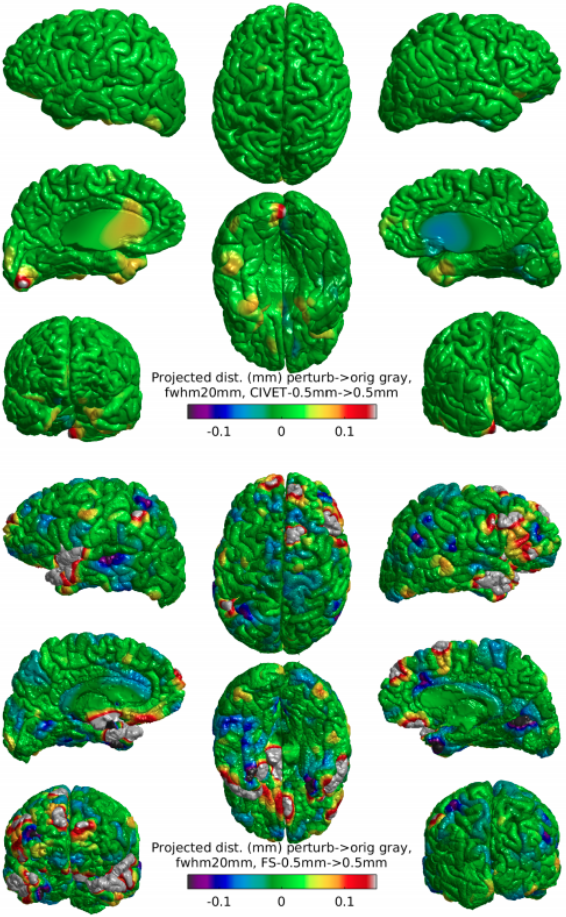
\includegraphics[width=0.6\textwidth]{./figs/onevoxel_civetfs.png}
\caption[Instability due to one-voxel perturbations]{Instability due to one-voxel perturbations of two cortical surface
estimation pipelines. Originally published with the following caption: Projected distance from perturbed to original
gray surface. Warm colors indicate that the original lies above the perturbed surface, while cool colors indicate that
the perturbed lies above the original surface. Green values near 0 are the ideal.~\cite{Lewis2017-ll}.}
\label{fig:onevox_cortical}
\end{figure}

The stability of neuroimaging pipelines has begun to be explored in specific use-cases through the perturbation of data
or libraries prior to processing. In the case of Diffusion MRI, the stability of tensor models were studied
analytically and validated experimentally~\cite{skare2000condition}. In this study, the stability of each tensor
reconstruction was first evaluated and found to contain considerable variability in stability across algorithms, ranging
from nearly $1$ (relatively stable) to nearly $10$ (highly unstable). The models were then tested across a range of
operating points, and showed a tight relationship between the observed variability and the theoretical
conditioning~\cite{skare2000condition}. Importantly, this work clearly demonstrated that experimental variability may
serve as a proxy for theoretical conditioning. This work also illustrated an often overlooked feature of variability: that
the stability of models varies across the space of inputs, and thus any evaluation of stability is inextricably linked to
both the tool and data being used.

Another exploration of stability through experimental perturbation compared two tools for cortical and sub-cortical
surface estimation~\cite{Lewis2017-ll} (Figure~\ref{fig:onevox_cortical}). In this experiment, grey matter surfaces were estimated from a single image using
two toolboxes. Subsequently, the intensity of a single voxel within the white matter (centre of the Corpus Callosum) of
the image was amplified by $1\%$ of its original value, and the tools were re-run. This analysis showed significant
differences between not only the original and perturbed surfaces, but showed non-uniformity in the variability across
cortical structures that was distinct for each tool~\cite{Lewis2017-ll}. This study importantly sheds light on the reality
that variability introduced to a workflow may affect the results in unexpected ways. The fact that the minor perturbation
of a single voxel buried within white matter may lead to a significant change in the estimation of grey matter matter
surfaces suggests that a more thorough exploration of perturbations and associated variability may be required to fully
understand the behaviour of these pipelines.

Though the magnitude of differences observed in the above cases is perhaps surprising, it may have been expected in all
scenarios to observe some non-zero amount of variability. However, differences in results have also been observed
in neuroimaging when changing operating system~\cite{Glatard2015-vc,salari2020file} or even padding an image with a row
of empty voxels~\cite{Glen2018-sg}. This array of findings clearly demonstrates the relevance of characterizing numerical
stability in the context of neuroimaging both due to the abundance of cases in which numerical inconsistencies have been
observed and the general lack of characterization of this effect. This thesis begins with enabling the rapid and
provenance rich deployment of neuroimaging workflows, and uses this platform to dig deep into the induction and
evaluation of numerical instabilities, the impact of instability on analytical workflows, and concludes with an
exploration of how the observed variability may be harnessed as a \textit{feature} rather than a bug.

